\documentclass[a4paper, 11pt, titlepage]{jsarticle}
\usepackage[dvipdfmx]{hyperref,graphicx}
\usepackage{listings}
\usepackage{amsmath}
\usepackage{url}
\usepackage{here}

\title{知能情報実験III(データマイニング班)\\Twitter上のテキスト文を対象とした「コロナで何が困っているのか」を見つける}
\author{グループの学籍番号 205759A, 205720E, 205763J, 195719J}
\date{提出日:2022年6月9日}
\begin{document}
\maketitle
\tableofcontents
\clearpage

\section{はじめに}

\subsection{分担}
zoomを使って、ペアプロのようにグループの全員でモデルの適用までのコーディングを進め、1通りの考察まで行った。最後の3週は役割分担して作業を進めた。以下に最後の3週の役割を示す。
205759A 比嘉和樹:コード、githubリポジトリの整理。
205720E 内藤武   :発表資料。モデルのドキュメント。
205763J 原田成斗:実験結果、考察。アクティビティ図の作成。
195719J:西村悠吾:レポートのデータセット構築。\_\_init\_\_.py(モジュール)の関数のドキュメント。


\subsection{概要}
グループ3は、Twitter 上のテキスト文を対象として「コロナで困っていること」を見つけることを対象問題として進めた。データセットとして、snscrapeを用いてtwitter上から「コロナ」という単語が含まれた25000件のツイートを取得した。このツイートをosetiと呼ばれるライブラリ関数を用いてネガティブかポジティブかの判定を行い、ネガティブだけのツイートを抽出した。集めたネガティブなツイートを用いて、形態素分析した。その結果をモデルに適用した。モデルは、教師なし学習で文書のクラスタリングを行うためLDA(トピックモデル) を使用した。また、トピックモデルはpyLDAvis を用いてインタラクティブに可視化した。

\subsection{テーマ:Twitter上のテキスト文を対象とした「コロナで何が困っているのか」を見つけるとは}
本グループではTwitter上のテキスト文を対象として「コロナで困っていること」を見つけることを対象問題として設定した。SNSを使ってコロナで発生している問題を可視化し、件数が多い項目を整理することで、その後の改善策を見出して今後に応用できる。それによって現在発生している問題に対処しつつ今後同様の問題が発生する際により効果的な対策ができるようになることが期待できる。

\section{実験方法}
\subsection{実験目的}
あるカテゴリに対するネガティブなツイートは、そのカテゴリによって「困っていること」だと判断する。したがって、今回のテーマである「コロナで困っていること」は、コロナというカテゴリについて述べているネガティブなツイート、すなわちコロナが含まれるツイートのうちネガティブなツイートをクラスタリングして得られた話題のことを指す。その得られた話題の中でもツイート数が多い話題は、より多くの人が困っている話題だと判断し、今回の実験ではそれを見つけることを目的とする。

\subsection{データセット構築}
以下にデータセット構築に必要なモジュールの中で定義した関数について箇条書きで説明する。\\
\noindent
Twitterscraping():Python のsnscrape ライブラリ・モジュールを使用して、ユーザー、ユーザープロファイル、ハッシュタグ、検索、ツイート(単一またはスレッド)、リスト投稿、トレンドから「コロナ」を含むテキストを取得する。件数(行数)は25,000件である。そして、それをデータフレームに変換する\cite{snscrape1}。その後、df.to\_csv()でテキストをカンマを区切り値としたcsvファイルに書き出す\cite{snscrape2}。\\
scraping\_results.csv:カンマを区切り値としたcsvファイル。UTF-8 Unicodeテキストで書かれており、非常に長い行(25000件)を持つ。スクレイピングした結果が保存されている。\\
extract\_content():pandas.read\_csv()でscraping\_results.csvをデータフレームとして読み込む\cite{snscrape3}。このデータフレームのうち、contentカラムの列だけで新たなデータフレームを作り、そのデータフレームをdf.to\_csv()でcsvファイルに書き出す。\\
contents.csv:カンマを区切り値としたcsvファイル。UTF-8 Unicodeテキストで書かれており、非常に長い行(25000件)を持つ。スクレイピングした結果のうち、ツイートとリツイートのテキストが保存されている。\\
judge(text):引数で渡されたテキストを、日本語評価極性辞書を利用したPython 用 Sentiment Analysis ライブラリoseti を使ってネガポジ判定()を行う\cite{negaposi1}。評価極性のスコアが 1 に近いほどポジティブで、 -1 に近いほどネガティブとなる。osetiを使ってネガポジ判定をしているサイトを参考にコードを書いた\cite{negaposi2}。\\
negaposi():pandas.read\_csv()でcontents.csvファイルをデータフレームとして読み込む。そして、データフレームに保存されているテキストを引数として、judge(text)を実行し、その戻り値を新たなカラムnegaposiに保存する。その後、negaposiカラムの値が 0 よりも大きい行を消し、新たなデータフレームを作る。そのデータフレームをdf.to\_csv()でcsvファイルに書き出す。\\
negative.csv:カンマを区切り値としたcsvファイル。UTF-8 Unicodeテキストで書かれている。ツイートとリツイートのテキストのうち、ネガティブと判定されたテキストが保存されている。\\
parse(tweet\_temp):形態素解析エンジンのMecabを使って、形態素解析をする\cite{keitaiso1}。まず、negative.csvのcontentカラムに保存されている値の1つ(1ツイート文)のすべての単語について辞書を通して形態素解析し、単語、品詞、品詞細分類、活用型、活用形、原形、読み、発音の情報を取り出して2次元リスト化する。情報がない部分には*を代入する。Mecabを使ってネガポジ判定をしているサイトを参考にコードを書いた\cite{keitaiso2}。\\
parse\_to\_df(tweet\_temp):negative.csvのcontentカラムに保存されている値の1つ(1ツイート文)をparse関数で形態素解析する。その後、カラムを形態素の種類ごとに設定したデータフレームを作成し、parse関数の結果を該当するカラムに保存する。作成したデータフレームを戻り値として返す。\\

\subsection{モデル選定}
実験目的に沿って、教師なし学習で文書のクラスタリングを行うためLDA(トピックモデル)を使用した。また、トピックモデルはpyLDAvisを用いてインタラクティブに可視化できる部分もLDAを選んだ理由である。 

\subsection{パラメータ調整}
クラスター数(カテゴリ数)の最適数を見つけるため、クラスター数3〜50の結果をメンバーで確認し、トピック名をつけやすいクラスター数を探した。また、その他のパラメータは参考にしたサイトの値をそのまま使用した\cite{LDA}。

\section{実験結果}
pyLDAvisを使用してトピックモデリングの内容をhtmlに出力した結果は以下の通りである。\href{https://ie.u-ryukyu.ac.jp/~e205759/pyldavis_output.html}{(リンク)}\\
 まず出力されたIntertopic Distance Mapの分布の見方から説明する。\\
\begin{figure}[H]
  \centering 
  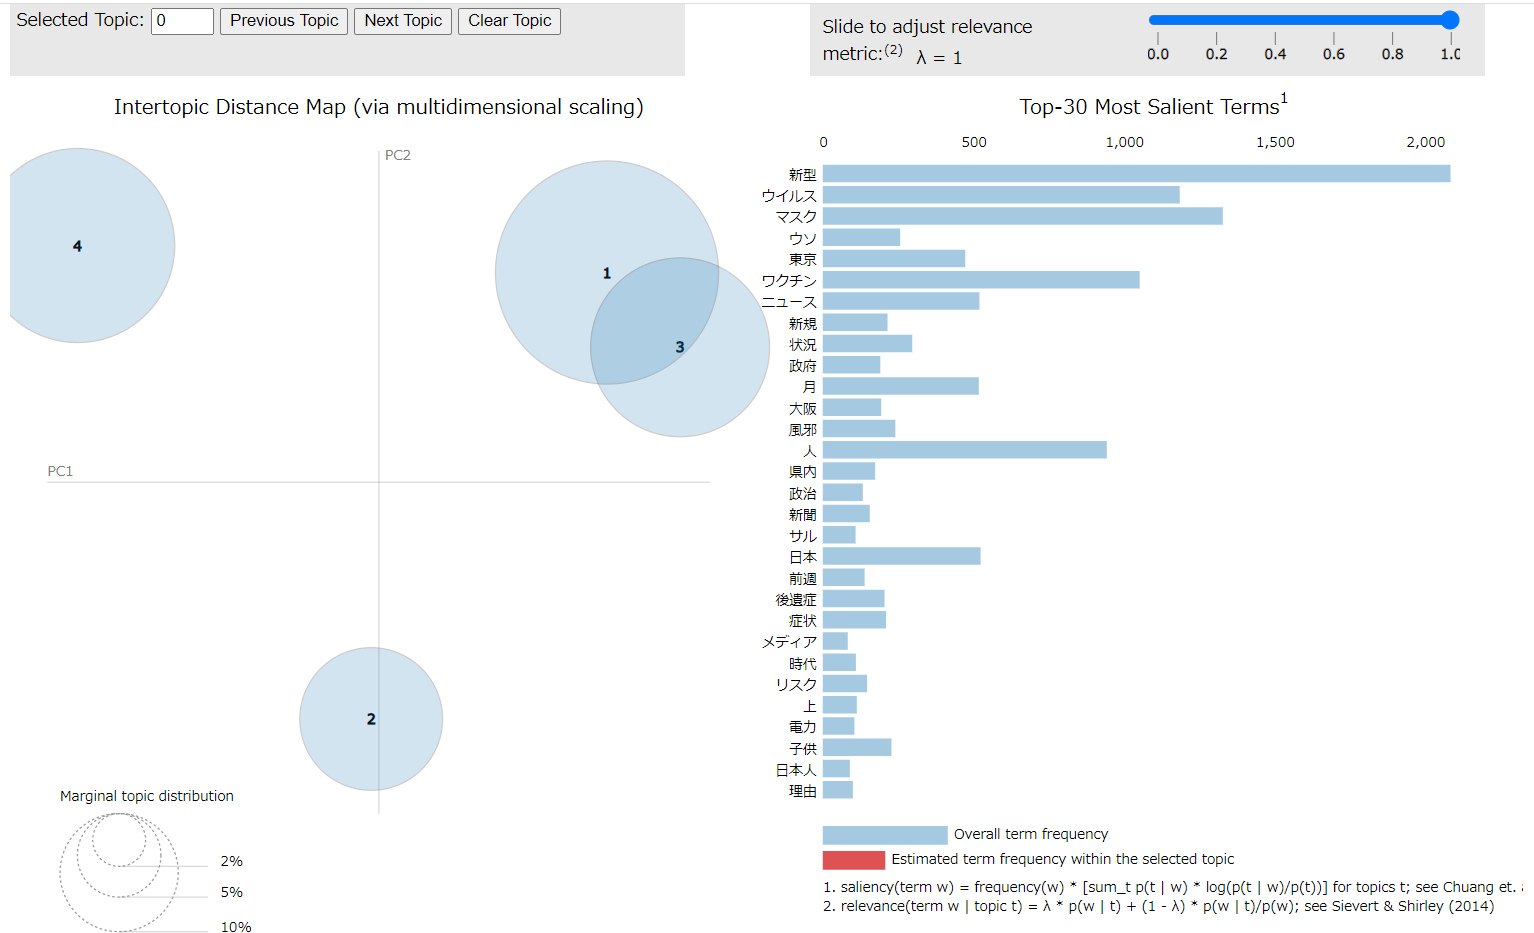
\includegraphics[scale=0.25]{picture1.png}
  \caption{トピックモデリングの出力結果}
\end{figure}
図1の左側には各トピックを多次元尺度法(MDS)で2次元に落として配置したものが表示され、円の大きさは全体の単語に対する、各トピックに所属する単語の割合を表している。また、右側には選択したトピックにおける頻出単語、同トピック内での出現頻度が大きい単語とその頻度が表示される。右上にあるパラメータλを変えると出現頻度、同トピック内での出現頻度の割合の比率を変えて順位を変えられる。右側の単語にマウスを重ねると各トピック内における出現頻度が左側の円の大きさとして表示される。\\
\newpage
図1によるとクラス1と3は似たトピックで、2と4はそれぞれ離れたトピックであることがわかる。また、全てのツイートに含まれている「コロナ」という単語を除くと、図2,3より、1と3のトピックで多く含まれる単語は「ワクチン」、「マスク」、「人」であり、また、「風邪」「症状」や「後遺症」という単語が1のトピックのみに含まれている。\\
\begin{figure}[H]
  \centering
  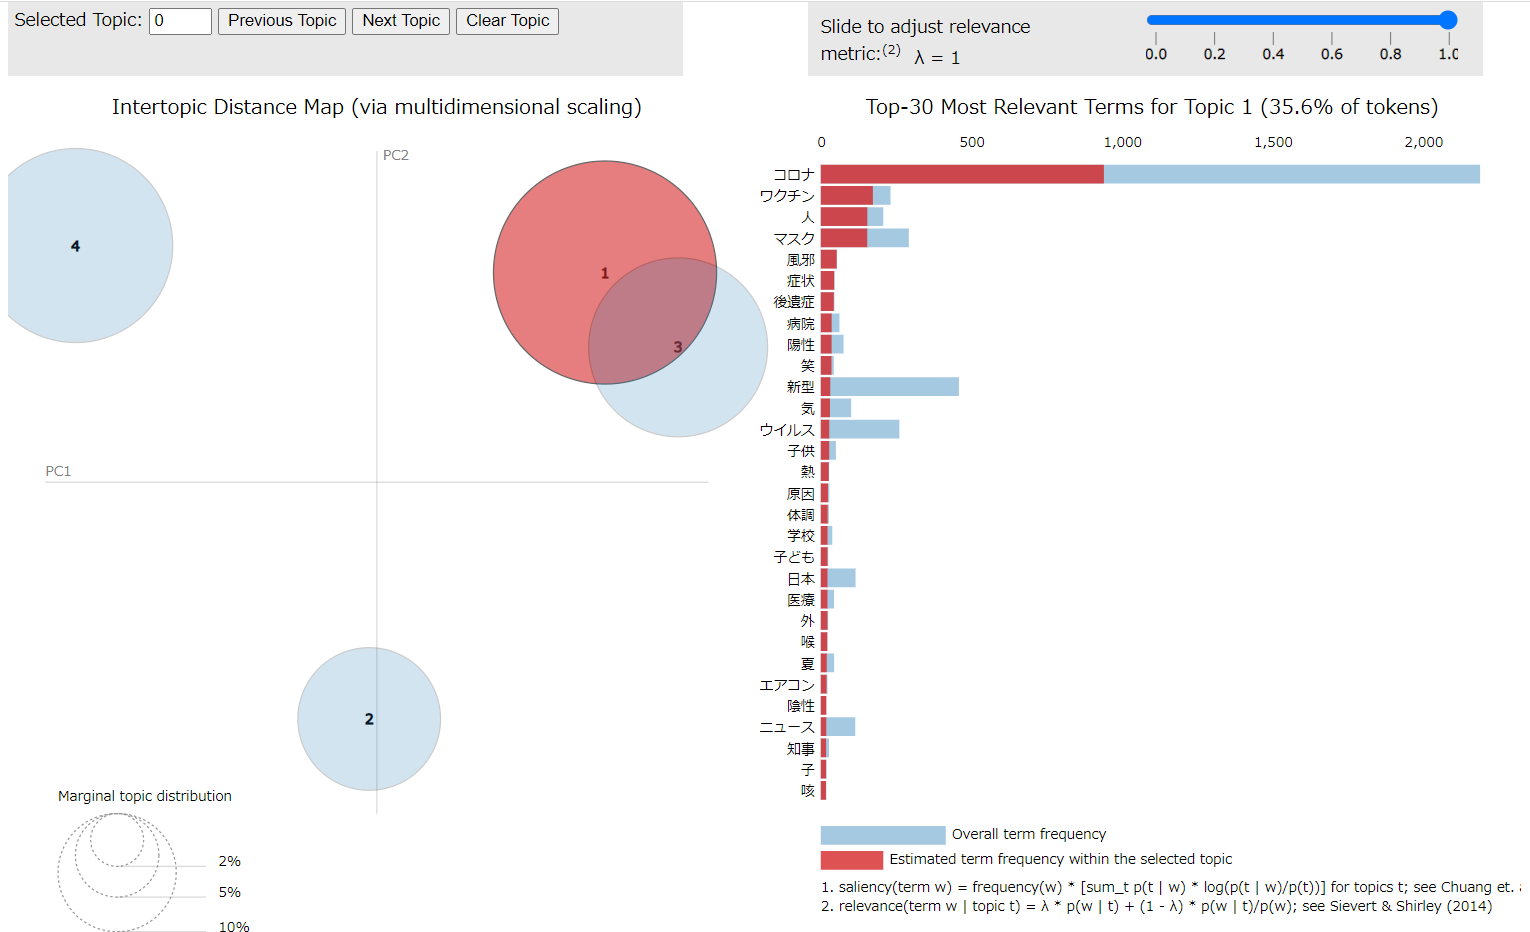
\includegraphics[scale=0.25]{picture2.png}
  \caption{クラス1の単語数}
  \centering
  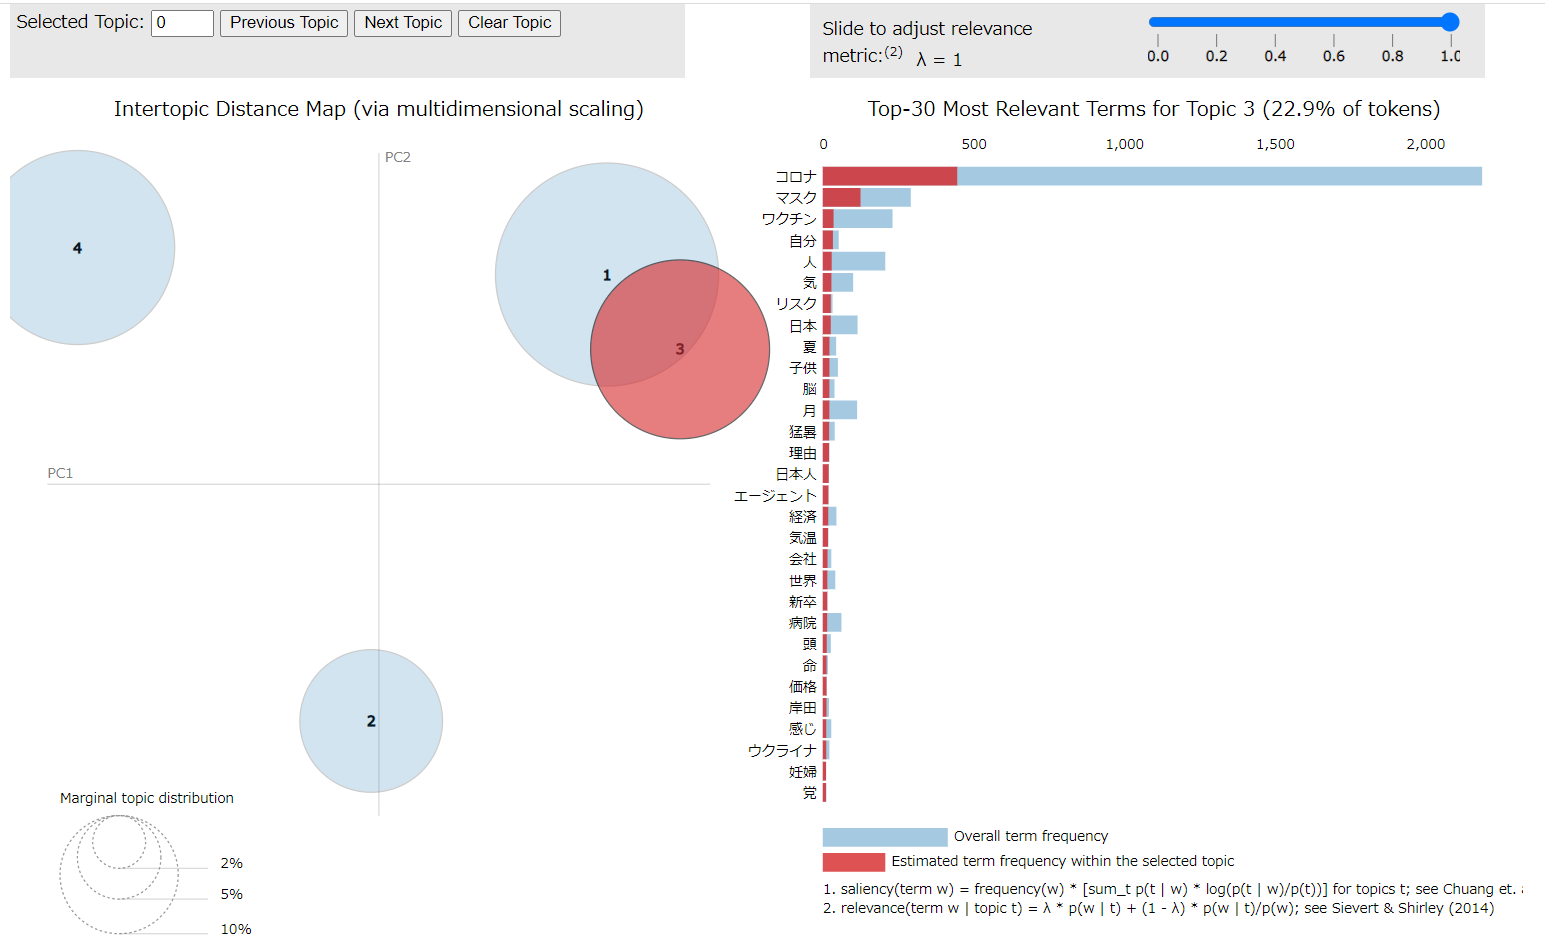
\includegraphics[scale=0.25]{picture3.png}
  \caption{クラス3の単語数}
\end{figure}
\newpage
図4を見ると、2のトピックで多い単語は「新型」「ウソ」「日本」であり、さらに、「政府」や「政治」という単語が多い。\\
\begin{figure}[H]
  \centering
  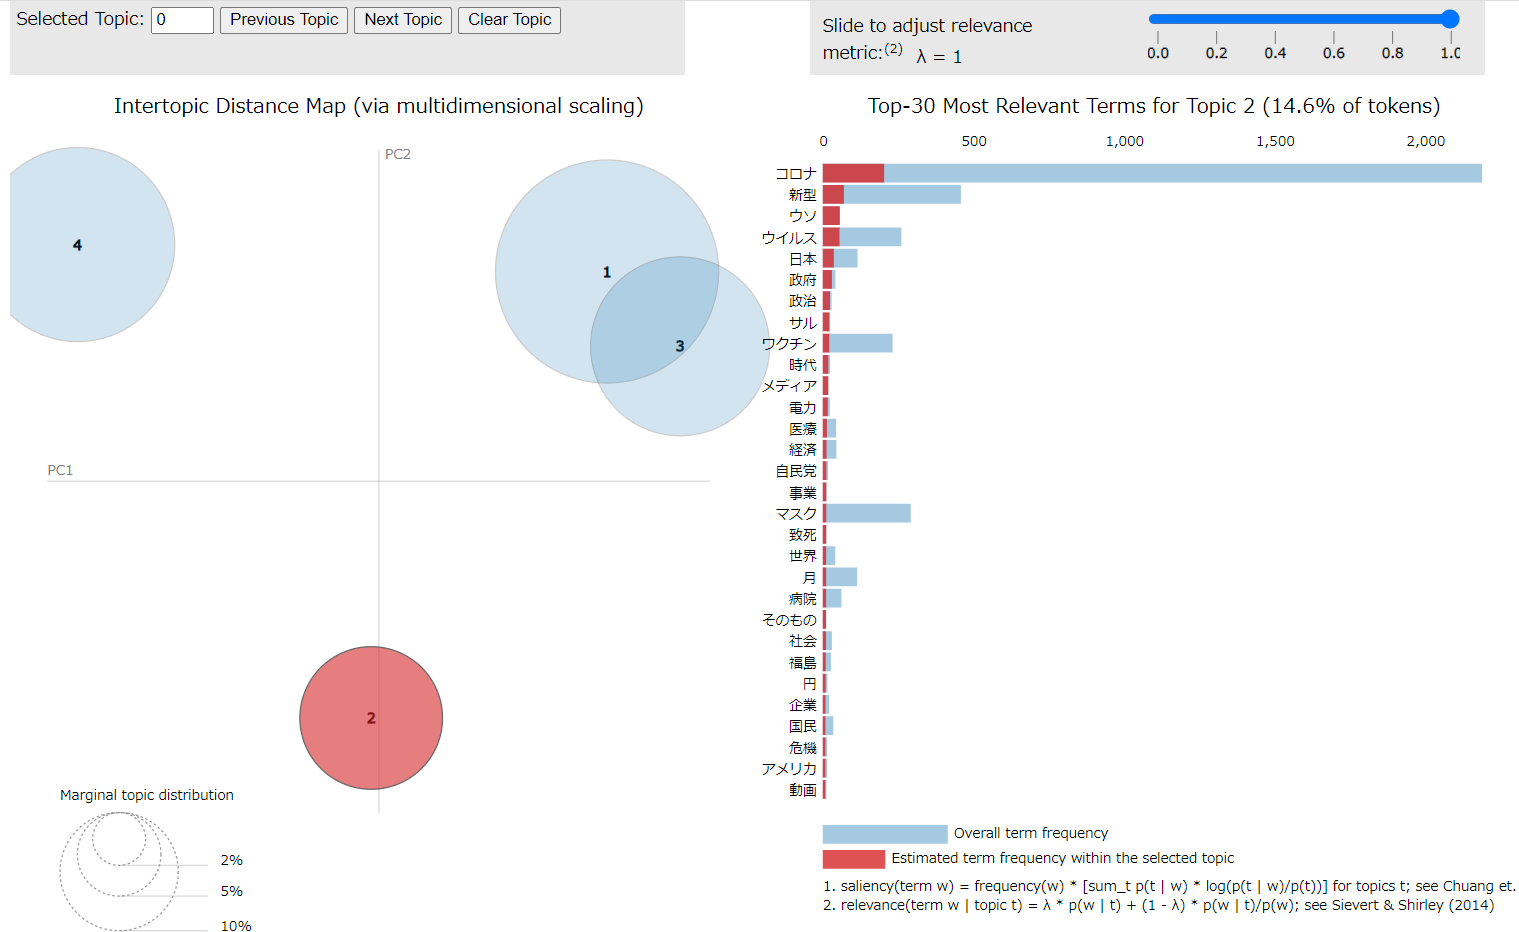
\includegraphics[scale=0.25]{picture4.png}
  \caption{クラス4の単語数}
\end{figure}
また、図5より4のトピックで多い単語は「新型」「ウイルス」「東京」であり、地名や「ニュース」、「新聞」といった単語が4のトピックに多いことがわかる。\\
\begin{figure}[H]
  \centering
  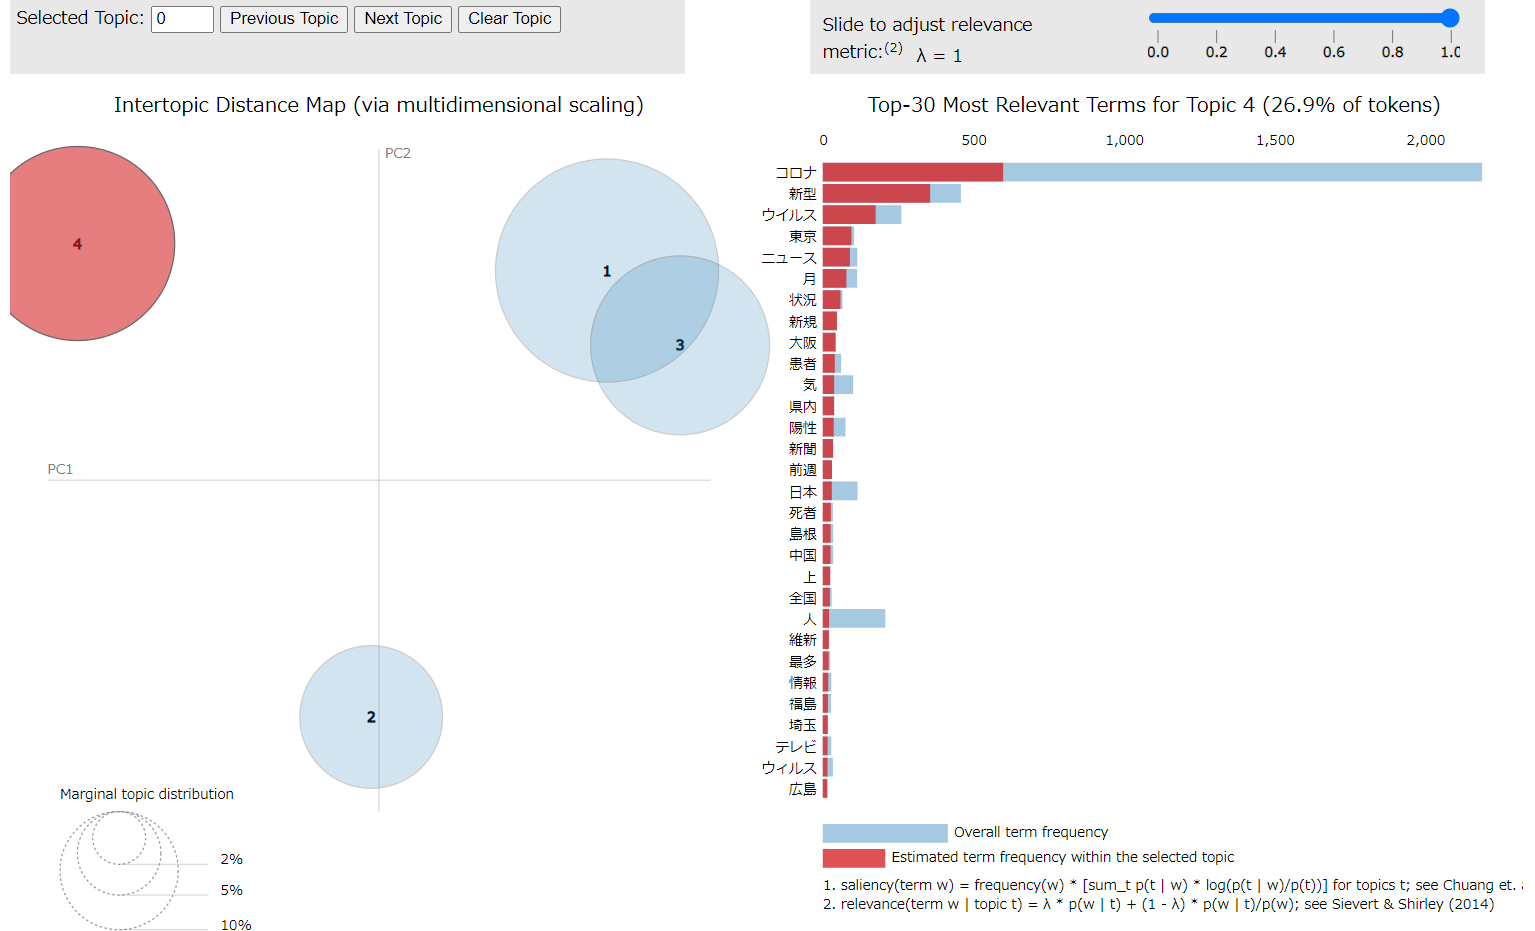
\includegraphics[scale=0.25]{picture5.png}
  \caption{クラス2の単語数}
\end{figure}

\section{考察}
実験結果より、トピック1,3は「コロナ感染症状」、トピック2は「政治」、トピック4は「メディア」の3つのトピックに分けられると考えた。さらに、今回データセットの構築を行う際「コロナ」という単語を含めたツイートを取得していたため、トピックごとに占めるコロナという単語数の割合が多いトピックが今回の実験目的に即していると考える。したがって、コロナによって困っていることのうち、改善する優先度の高いトピックは、コロナ感染症状、ニュース、政治の順であると考える。\\

 また、今回の実験は参考資料をもとに行っていたため、LDAのパラメータを理解し、調整するなどを行えていない。今後、より今回の実験に合わせたモデルの構築を行うことができればより良い結果が出るのではないかと考える。また、データの数としてネガティブとして判定されたツイート数は約1万件だった。今回の実験としてこのデータ数が最適なのかということも考えなければならない。

\subsection{追加実験}
(まだ実験していないので書いていません。)

\section{意図していた実験計画との違い}


\section{まとめ}
目標としていた「コロナで困っていることの抽出」について、実験用のプログラム作成には成功したものの抽出した内容は具体性に乏しく、達成には至らなかった。
pyLDAvisによる結果の可視化の重要性が理解できた。
Mecabとgensim\_modelsを利用して簡単にトピックモデリングができ、日本語極性辞書のosetiによるネガポジ判定は人の目にも精度が高かったため、優秀なライブラリが多いというpythonの長所を実感した。

\begin{thebibliography}{n}
  \bibitem{kanazawa}レポート作成の手引き レポートの基本的形式に関するガイド, \url{https://www.kanazawa-u.ac.jp/wp-content/uploads/2015/01/tebiki2.pdf}, 2022/07/28.
      \bibitem{snscrape1}snscrape, \url{https://github.com/JustAnotherArchivist/snscrape}, 2022/07/28.
      \bibitem{snscrape2}pandas documentation, \url{https://pandas.pydata.org/docs/reference/api/pandas.DataFrame.to_csv.html}, 2022/07/28.
      \bibitem{snscrape3}pandas documentation, \url{https://pandas.pydata.org/docs/reference/api/pandas.read_csv.html#pandas.read_csv}, 2022/07/28.
      \bibitem{negaposi1}日本語評価極性辞書を利用したPython用Sentiment Analysisライブラリ oseti を公開しました, \url{https://qiita.com/yukinoi/items/46aa016d83bb0e64f598}, 2022/07/28.
      \bibitem{negaposi2}osetiによる日本語の感情分析, \url{https://note.com/npaka/n/n3c7722d2e4bc}, 2022/07/28
      \bibitem{keitaiso1}MeCab: Yet Another Part-of-Speech and Morphological Analyzer, \url{https://taku910.github.io/mecab/}, 2022/07/28.
      \bibitem{keitaiso2}Mecab(形態素解析)で遊んでみた!, \url{https://qiita.com/str32/items/c1ced3b017ff5cacc4dc}, 2022/07/28.
      \bibitem{LDA}Shingoの数学ノート, \url{http://mathshingo.chillout.jp/blog27.html}, 2022/07/28.

\end{thebibliography}
\end{document}
